\documentclass{classrep}
\usepackage[utf8]{inputenc}
\frenchspacing

\usepackage{graphicx}
\usepackage[usenames,dvipsnames]{color}
\usepackage[hidelinks]{hyperref}
\usepackage{subfig}

\usepackage{amsmath, amssymb, mathtools}

\usepackage{fancyhdr, lastpage}
\pagestyle{fancyplain}
\fancyhf{}
\renewcommand{\headrulewidth}{0pt}
\cfoot{\thepage\ / \pageref*{LastPage}}


\studycycle{Informatyka, studia dzienne, I st.}
\coursesemester{IV}

\coursename{Inteligentna Analiza Danych}
\courseyear{2016/2017}

\courseteacher{mgr inż. Paweł Tarasiuk}
\coursegroup{piątek, 12:00}

\author{%
  \studentinfo[203943@edu.p.lodz.pl]{Jakub Mielczarek}{203943}\\
  \studentinfo[203882@edu.p.lodz.pl]{Łukasz Gołębiewski}{203882}%
}

\title{Zadanie 2.: Perceptron wielowarstwowy}

\begin{document} 
\maketitle 
\thispagestyle{fancyplain}

\section{Cel}
{\color{black}
Przedmiotem zadania jest implementacja perceptronu wielowarstwowego o charakterze uniwersalnym, gdzie jako metodę jego nauki zastosowaliśmy algorytm wstecznej propagacji błędów.

\section{Wprowadzenie}
{\color{black}
Uniwersalność perceptronu oznacza, iż wszystkie parametry sieci neuronowej, takie jak liczba warstw, liczba neuronów w danej warstwie, współczynnik nauki, momentum czy parametr decydujący czy neurony mają uwzględniać wartość wejścia obciążającego (bias) są przekazywane w postaci argumentów, co pozwala badać zachowanie różnych konfiguracji. 
Wyróżniamy 3 typy warstw: warstwę wejściową(nieprzetwarzającą), dowolną liczbę warstw ukrytych(nieliniowych) oraz warstwę wyjściową(nieliniową). Zawierają one neurony. Każdy neuron posiada dowolną liczbę wejść oraz jedno wyjście, które jednak może trafiać na kilka wejść neuronów kolejnej warstwy. Nieliniowość warstwy oznacza zastosowanie w naszym zadaniu sigmoidalnej funkcji aktywacji:
\begin{equation}
sig(x) = \dfrac{1}{1+e^{-x}}
\end{equation}
Poniżej przedstawimy metodę pozwalającą obliczyć wyjścia wszystkich warstw na podstawie zadanego wejścia:\\
1. Obliczamy sumę ważoną wejść neuronu:
\begin{equation}
sum = {\sum_{i=0}^{n} (w_i * v_i)} 
\end{equation}
$w_{i}  - waga \quad i-tego \quad wejscia $
\\
$v_{i}  - wartosc \quad i-tego \quad wejscia $\\
2. Obliczamy wyjście neuronu wykorzystując funkcję aktywacji(1):
\begin{equation}
out = sig(sum+bias)
\end{equation}
\\
Procesem o zdecydowanie większej złożoności jest metoda wstecznej propagacji błędów. Jak sugeruje sama nazwa algorytmu proces ten polega na policzeniu błędu każdego z neuronów poczynając od neuronów wyjściowych:
\begin{equation}
\Delta_{last} = (out - v_i) * sig'(sum)
\end{equation}
Błąd dla neuronów pozostałych (poprzednich) warstw obliczamy ze wzoru:
\begin{equation}
\Delta = sig'(x) * \sum_{j=0}^{m} (\Delta_{next} * w_{j})
\end{equation}
Po obliczeniu błędów dla każdej warstwy nieliniowej przechodzimy do ostatniego etapu, czyli modyfikacji wag:
\begin{equation}
w_{i}^{curr} = learningRate * \Delta * v_{i} + momentum * (w_{i}^{curr} - w_{i}^{prev})
\end{equation}
Momentum oraz learningRate to parametry podawane przez użytkownika na starcie programu.
\\
Warunkiem kończącym proces nauki jest w naszym programie osiągnięcie odpowiedniej epoki, których liczba jest przekazywana jako parametr.
\\
Program generuje dwa wykresy będące podstawą do podjęcia dyskusji i wyciągnięcia odpowiednich wniosków. Pierwszy z nich zawiera zestawienie obliczonych wyjść względem oczekiwanych wartości. Drugi przedstawia błąd sieci będący kwadryką różnicy między wejściami obliczonymi a oczekiwanymi.
}

\section{Opis implementacji}
Podstawowy opis plików klas:
\begin{itemize}
	\item Layer.java - klasa, której instancja reprezentuje warstwę neuronową (przechowuje neurony oraz informacje o ich liczbie)
	\item Neuron.java - klasa reprezentująca pojedynczy neuron 
	\item MultiLayerPerceptron.java - główny moduł programu, klasa odpowiadająca za utworzenie perceptronu oraz implementacja metod modyfikujących stan neuronów
	\item MlpCli.java - main, dodatkowo dostarcza interfejs CLI
	\item ActivationFunction.java - interfejs 	
	\item Sigmoidal.java - implementacja sigmoidalnej funkcji aktywacji
	\item MLPUtils.java - klasa pomocnicza zawierająca statyczne metody do operacji takich jak obliczenie kwadryki, serializacja, zapis wyników do pliku
\\

Program, który wykorzystaliśmy do rysowania wykresów to Gnuplot.
Lista uruchomieniowa programu została zaprojektowana zgodnie z wytycznymi zawartymi w instrukcji do zadania. Opis parametrów wraz z przykładowym wywołaniem prezentujemy poniżej:

\begin{figure}[h!]
\centering
 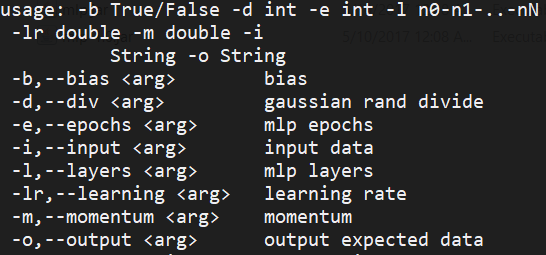
\includegraphics{img/arg.png}
 \vspace{-0.3cm}
\end{figure}

\end{itemize}
\newpage
\section{Materiały i metody}
Część badawcza 1 polega na nauce perceptronu 4 poniższych wzorców: \\
IN  $\Rightarrow$ OUT \\
1 0 0 0 $\Rightarrow$ 1 0 0 0 \\
0 1 0 0 $\Rightarrow$ 0 1 0 0 \\
0 0 1 0 $\Rightarrow$ 0 0 1 0 \\
0 0 0 1 $\Rightarrow$ 0 0 0 1 \\
Zbadamy wpływ uwzględnienia obciążenia w neuronach nieliniowych na skuteczność nauki powyższych wzorców. Następnie zbadamy zachowanie wersji perceptronu, dla której uzyskaliśmy zbieżność,  przy różnych wartościach współczynnika nauki oraz momentum określonych w treści zadania.\\
\\
Część badawcza 2 polega na realizacji funkcji logicznej XOR: \\
IN  $\Rightarrow$ OUT \\
0 0 $\Rightarrow$ 0 \\
0 1 $\Rightarrow$ 0 \\
1 0 $\Rightarrow$ 0 \\
1 1 $\Rightarrow$ 1 \\
Zbadamy możliwość uczenia się sieci neuronowej dla układu nie wykazującego separowalności liniowej. Oznacza to, iż nie da się wyznaczyć prostej linii dzielącej przestrzeń danych na dwie mniejsze, z których jedna odpowiada sygnałowi '1' na wyjściu, a druga '0' na wyjściu. Niemożliwym jest rozwiązanie tego problemu przy użyciu jednego perceptronu. Wyjściem z sytuacji jest dodanie przynajmniej jednego neuronu w warstwie ukrytej, co pozwoli zrealizować oczekiwany podział przestrzeni.

 }

\newpage
\section{Wyniki}
{
\subsection{Część badawcza 1} 

IN 1 0 0 0 $\Rightarrow$ OUT 1 0 0 0\\
LAYER 2\\
Neuron 0: Weights: -3.64 -1.50 -1.50 4.65 Value: 0.03\\
Neuron 1: Weights: 4.65 -1.50 -1.51 -3.67 Value: 0.99 \\
LAYER 3 \\
Neuron 0: Weights: -13.73 2.90 Value: 0.93\\
Neuron 1: Weights: -1.92 -1.92 Value: 0.12 \\
Neuron 2: Weights: -1.93 -1.92 Value: 0.12 \\
Neuron 3: Weights: 2.89 -13.74  Value: 0.00 \\

\begin{figure}[h!]
 \centering
 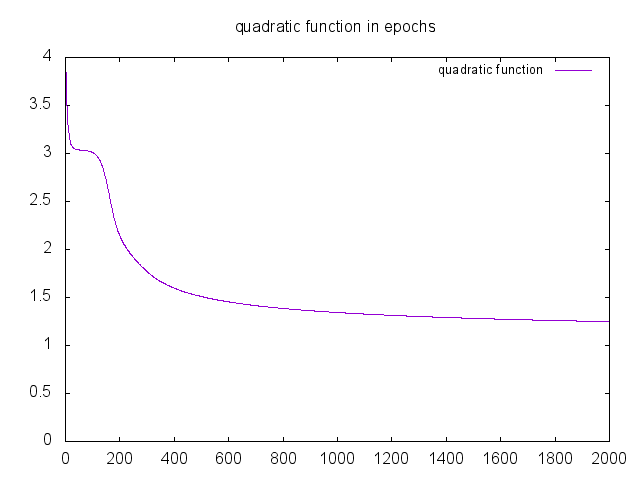
\includegraphics[width=12cm]{img/424biasfalse.png}
 \vspace{-0.3cm}
 \caption{java -jar mlp.jar -b False -d 25 -e 2000 -l 4-2-4 -lr 0.6 -m 0.0 -i dataz2in.data -o data/z2out.data }
\end{figure}

 
\begin{figure}[h!]
 \centering
 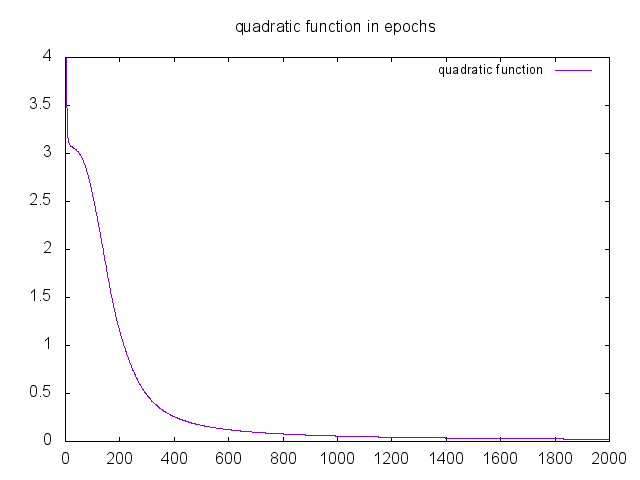
\includegraphics[width=12cm]{img/424biastrue.png}
 \vspace{-0.3cm}
 \caption{java -jar mlp.jar -b True -d 25 -e 2000 -l 4-2-4 -lr 0.6 -m 0.0 -i data/z2in.data -o data/z2out.data}
\end{figure}

\newpage

\begin{figure}[h!]
 \centering
 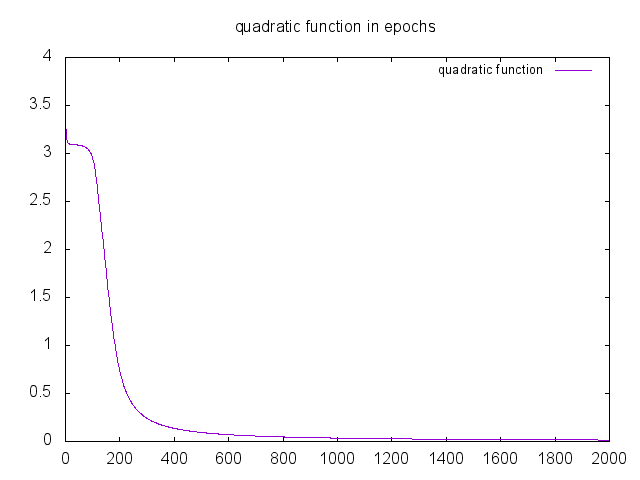
\includegraphics[width=12cm]{img/424lr09.png}
 \vspace{-0.3cm}
 \caption{java -jar mlp.jar -b True -d 25 -e 2000 -l 4-2-4 -lr 0.9 -m 0.0 -i data/z2in.data -o data/z2out.data}
\end{figure}

\begin{figure}[h!]
 \centering
 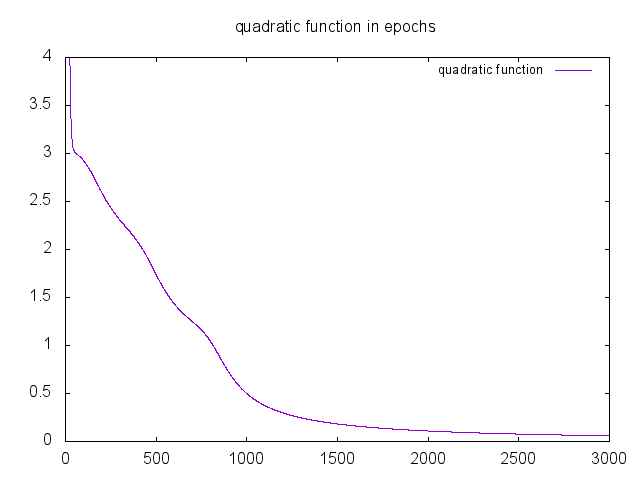
\includegraphics[width=12cm]{img/424lr02.png}
 \vspace{-0.3cm}
 \caption{java -jar mlp.jar -b True -d 25 -e 3000 -l 4-2-4 -lr 0.2 -m 0.0 -i data/z2in.data -o data/z2out.data}
\end{figure}

\newpage

\begin{figure}[h!]
 \centering
 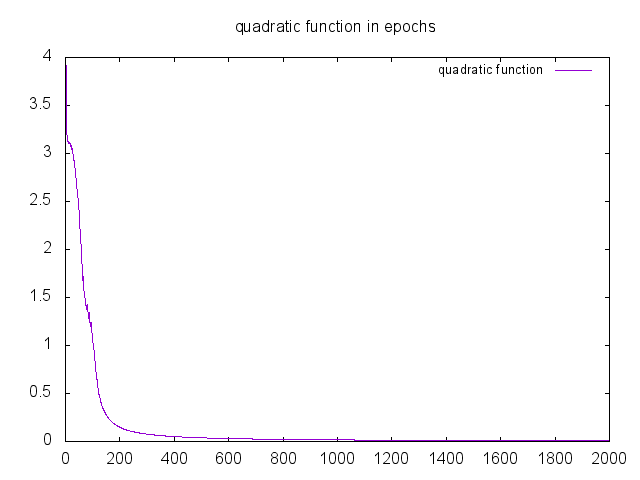
\includegraphics[width=12cm]{img/424lr09m06.png}
 \vspace{-0.3cm}
 \caption{java -jar mlp.jar -b True -d 25 -e 2000 -l 4-2-4 -lr 0.9 -m 0.6 -i data/z2in.data -o data/z2out.data}
\end{figure}

\newpage
\begin{figure}[h!]
 \centering
 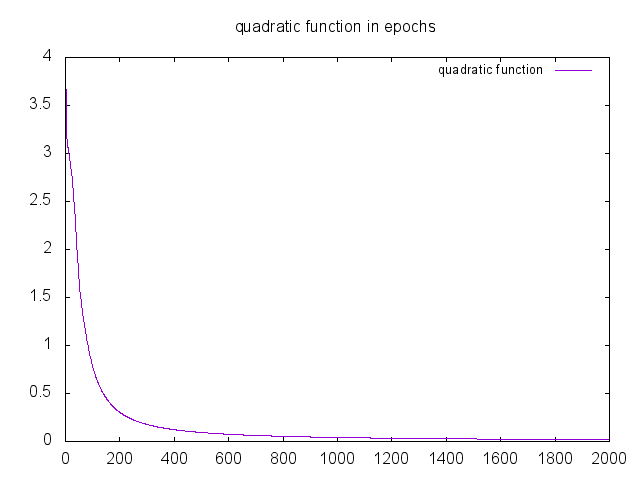
\includegraphics[width=12cm]{img/424lr02m09.png}
 \vspace{-0.3cm}
 \caption{java -jar mlp.jar -b True -d 25 -e 2000 -l 4-2-4 -lr 0.2 -m 0.9 -i data/z2in.data -o data/z2out.data}
\end{figure}

\subsection{Część badawcza 2}
\begin{figure}[h!]
 \centering
 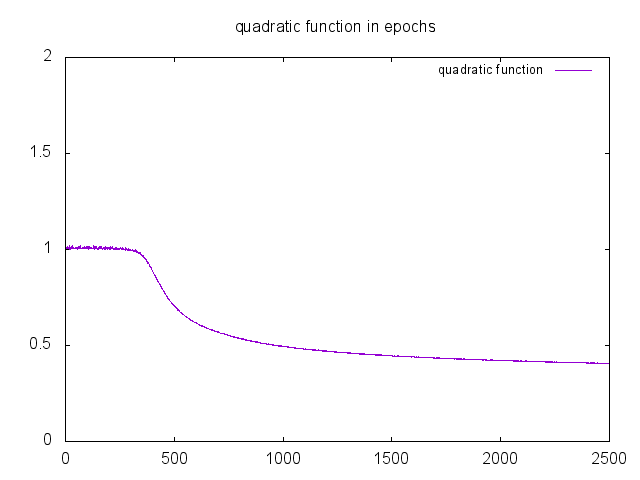
\includegraphics[width=12cm]{img/xor221biasfalse.png}
 \vspace{-0.3cm}
 \caption{java -jar mlp.jar -b False -d 25 -e 2500 -l 2-2-1 -lr 0.2 -m 0.8 -i data/xorin.data -o data/xorout.data}
\end{figure}

\newpage
\begin{figure}[h!]
 \centering
 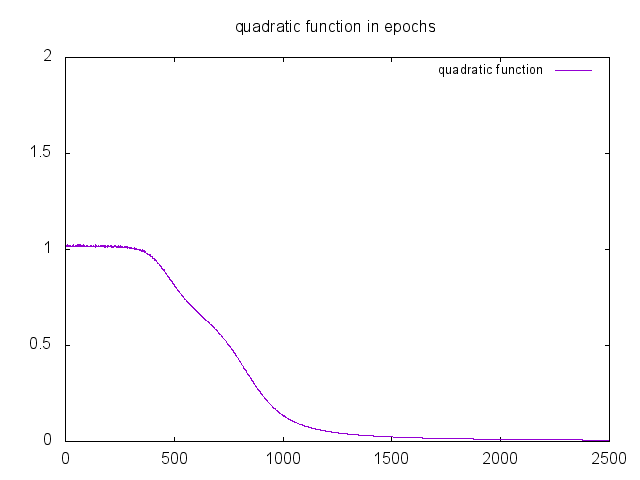
\includegraphics[width=12cm]{img/xor221biastrue.png}
 \vspace{-0.3cm}
 \caption{java -jar mlp.jar -b True -d 25 -e 2500 -l 2-2-1 -lr 0.2 -m 0.8 -i data/xorin.data -o data/xorout.data}
\end{figure}

\begin{figure}[h!]
 \centering
 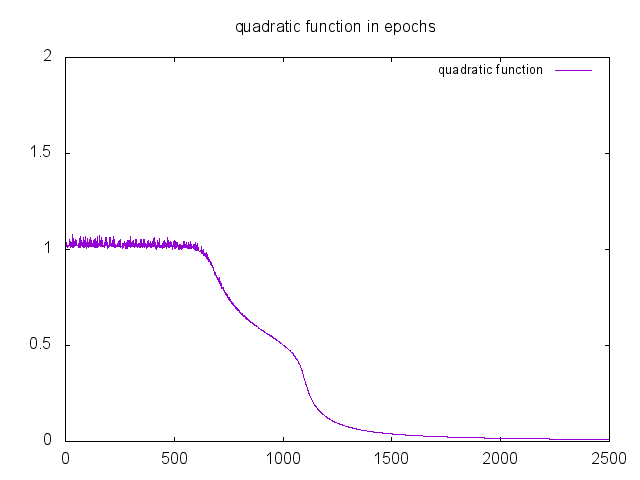
\includegraphics[width=12cm]{img/xor261.png}
 \vspace{-0.3cm}
 \caption{java -jar mlp.jar -b True -d 25 -e 2500 -l 2-6-1 -lr 0.2 -m 0.8 -i data/xorin.data -o data/xorout.data}
\end{figure}

\section{Dyskusja i wnioski}
{
\subsection{Część badawcza 1}
Dwie pierwsze badane konfiguracje miały odpowiedzieć na pytanie czy obecność biasu ma wpływ na autoasocjacje perceptronu o strukturze 4-2-4. Stwierdzamy, że użycie biasu jest dla tej konfiguracji konieczne do uzyskania zbieżności. Zauważamy również niemal identyczne wartości uzyskane dla 2 i 3 neuronu (Przypadek 1), co pozwala przypuszczać, iż wejścia te są nierozróżnialne dla naszej sieci.
\\
Kolejne konfiguracje przedstawiały sieci z uwzględnionym obciążeniem, jednak dla różnych ustawień parametrów nauki oraz momentum. Pierwszym oczywistym wnioskiem jest fakt, iż ustawienie tych parametrów na wartości większe od 1 prowadzi do rozbieżności. Posiłkując się wykresami zauważamy, że im wyższe wartości parametrów, tym szybciej uzyskujemy zadowalające rezultaty (Rysunek 5). Opierając swoją wiedzę tylko na wykresach nie jesteśmy w stanie określić, który z tych parametrów pełni ważniejszą rolę dla algorytmu, gdyż wysoka wartość jednego z nich przy marignalnym wpływie drugiego (i odwrotnie) pozwoliła uzyskać niemal identyczne wyniki (Rysunki 3 i 6 - zbieżność w granicach 1500 epoki). Jednak analizując powyższe wzory stwierdzamy, że niemożliwą jest nauka perceptronu dla współczynnika nauki równego 0, natomiast udowodniliśmy, że brak momentum wpływa jedynie na jakość przeprowadzanego procesu (Rysunki 2,3,4), nie decydując o jego powodzeniu.
Dodatkowo w nieudokumentowanych tutaj przypadkach zauważono, że konieczne losowanie początkowych wag z małego przedziału wartości oscylującego wokół zera. Jeśli ten warunek nie jest spełniony sieć uzyskuje złe rezultaty. Gorsze wyniki sieć uzyskuje również gdy danie podawane w każdej epoce będą w tej samej kolejności dlatego po każdej epoce uczenia kolejność danych wejściowych jest losowana. 
\\
Podsumowując obecność biasu odgrywa kluczową rolę dla powodzenia nauki prostej sieci zawierającej niewielką liczbę neuronów. Momentum pozwala przyspieszyć proces uczenia.


\subsection{Część badawcza 2}
Pierwsza i druga (Rys.7-8) badana konfiguracja o strukturze 2-2-1 potwierdza tezę o decydującym wpływie biasu dla sieci o tak prostej budowie (pomimo sprzyjających wartości współczynników). Trzecia (Rys. 3) pokazuje, że brak biasu można rozwiązać poprzez dodanie większej liczby neuronów w warstwie ukrytej. 



\end{document}
